\documentclass[11pt]{article}
\usepackage{amsmath, amssymb}
\usepackage{booktabs}
\usepackage{graphicx}
\usepackage{hyperref}
\usepackage{geometry}
\geometry{margin=1in}

\title{Homework 1 --- Questions 4 \& 5}
\date{}

\begin{document}
\maketitle

% ─────────────────────────────────────────────
\section*{Question 4: Normality of Residuals}
% ─────────────────────────────────────────────

To evaluate whether square error loss is justified for the Average Localization
Error (ALE) dataset, we fit four regression models --- Linear Regression, SVM,
Decision Tree, and Neural Network --- and examined the normality of their
residuals using QQ plots and the \texttt{normaltest} from \texttt{scipy}. As
shown in Figure~\ref{fig:qqplots}, the Linear Regression and SVM models both
produced residuals that are mostly normally distributed, with points following
the reference line closely in the middle range while deviating at the tails.
The Neural Network produced the most normally distributed residuals among all
models, with points adhering tightly to the reference line across almost the
entire range with only minor tail deviations. The Decision Tree, however,
produced residuals of essentially zero due to perfect overfitting of the
training data, rendering the normality test meaningless.

\begin{figure}[h]
    \centering
    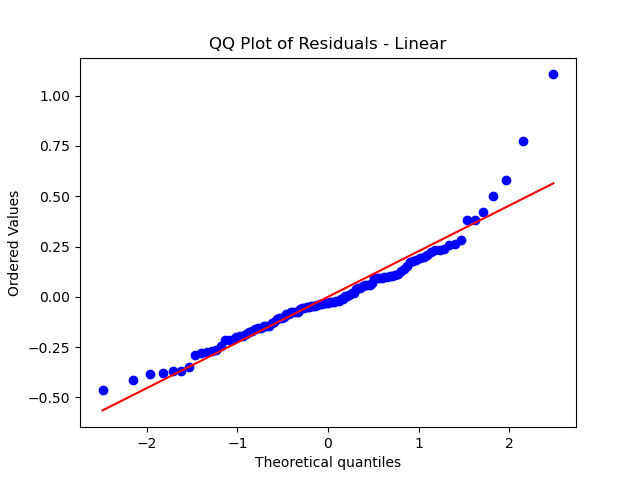
\includegraphics[width=0.45\textwidth]{Figure_1_linear.png}
    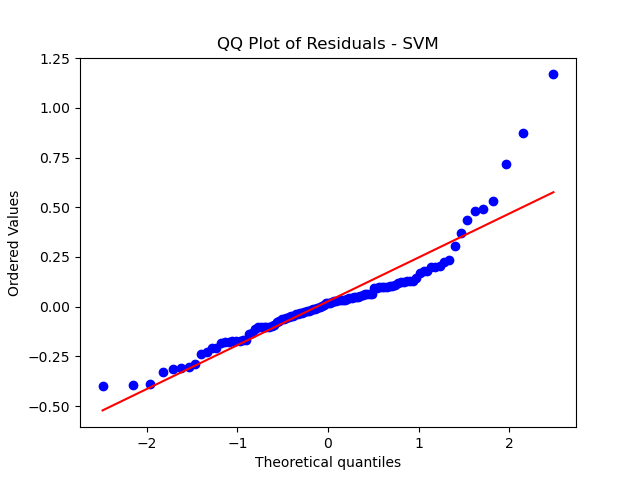
\includegraphics[width=0.45\textwidth]{Figure_2_SVM.png}

    \vspace{0.5em}

    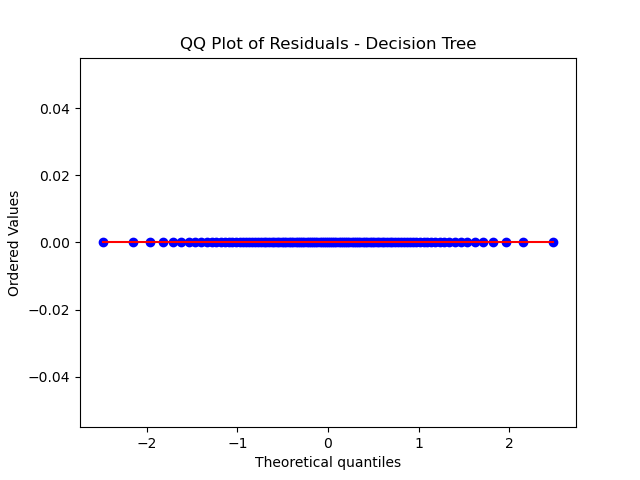
\includegraphics[width=0.45\textwidth]{Figure_3_Decision_Tree.png}
    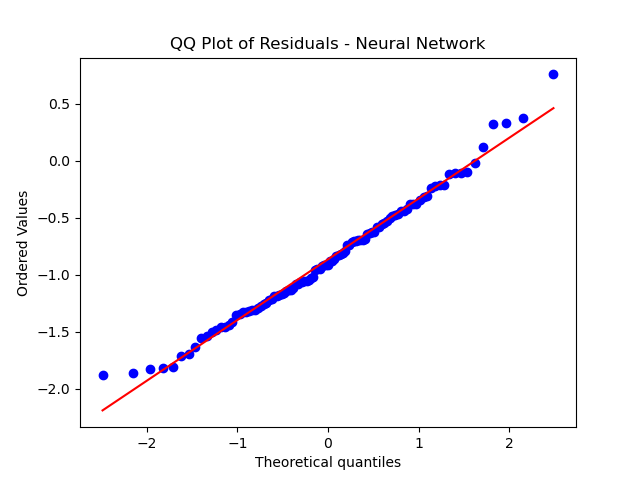
\includegraphics[width=0.45\textwidth]{Figure_4_Neural_Network.png}

    \caption{Q-Q plots of residuals for different regression models.
             (a) Linear Regression, (b) SVM, (c) Decision Tree, (d) Neural Network.}
    \label{fig:qqplots}
\end{figure}

To further quantify the normality of the residuals, we report the $p$-values
from the \texttt{normaltest} in Table~\ref{tab:normality}. The Linear
Regression and SVM returned very small $p$-values of $1.287 \times 10^{-9}$
and $1.615 \times 10^{-12}$ respectively, meaning we \textbf{reject} the null
hypothesis of normality for both models at any conventional significance level.
The Neural Network returned a $p$-value of $0.2367$, which is well above the
$0.05$ threshold, meaning we \textbf{fail to reject} normality --- its
residuals are statistically consistent with a normal distribution. The Decision
Tree returned \texttt{NaN} due to perfect overfitting. Overall, only the Neural
Network satisfies the normality assumption, providing the strongest
justification for the use of square error loss among the four models tested.

\begin{table}[h]
    \centering
    \caption{Normality test results for model residuals.}
    \label{tab:normality}
    \begin{tabular}{lc}
        \toprule
        \textbf{Model} & \textbf{$p$-value} \\
        \midrule
        Linear Regression & $1.287 \times 10^{-9}$  \\
        SVM               & $1.615 \times 10^{-12}$ \\
        Decision Tree     & \texttt{NaN}            \\
        Neural Network    & $0.2367$                \\
        \bottomrule
    \end{tabular}
\end{table}

% ─────────────────────────────────────────────
\section*{Question 5: Automatic Differentiation}
% ─────────────────────────────────────────────

\subsection*{Classification (Breast Cancer Wisconsin Dataset)}

The Breast Cancer Wisconsin dataset contains 569 observations with 30 features
and a binary label. We split the data 80/20 into training (455 samples) and
test (114 samples) sets, and standardized all features using
\texttt{StandardScaler} fit on the training set only.

\paragraph{Baseline.}
A scikit-learn \texttt{LogisticRegression} model (max\_iter$=1000$) trained on
the scaled features achieved a test accuracy of $\mathbf{0.9825}$.

\subsubsection*{Part (a): Custom Logistic Regression}

We implemented a logistic regression model in PyTorch:
\[
    f(x_i) = \sigma(w^\top x_i + b),
    \qquad
    \sigma(z) = \frac{1}{1 + e^{-z}},
\]
with binary cross-entropy loss:
\[
    L(y_i, f(x_i)) = -\bigl[y_i \log f(x_i) + (1-y_i)\log(1-f(x_i))\bigr].
\]
Predicted probabilities were clipped to $[\varepsilon,\, 1-\varepsilon]$ with
$\varepsilon = 10^{-7}$ to avoid evaluating $\log(0)$. The model was trained
for 5{,}000 epochs using \texttt{torch.optim.SGD} with learning rate $0.01$.
Training loss decreased steadily from $0.6931$ at epoch~0 to $0.0659$ at
epoch~4500, indicating stable convergence. The custom logistic regression
achieved a test accuracy of $\mathbf{0.9737}$, which is $0.9\%$ below the
sklearn baseline, a small gap attributable to the approximate nature of SGD
compared to sklearn's exact solver.

\subsubsection*{Part (b): Probit Regression}

Probit regression replaces the sigmoid link function with the standard normal
cumulative distribution function $\Phi$:
\[
    f(x_i) = \Phi(w^\top x_i + b).
\]
The same binary cross-entropy loss, clipping strategy, and SGD optimizer
(lr$=0.01$, 5{,}000 epochs) were used. Training loss decreased from $0.6931$
at epoch~0 to $0.0554$ at epoch~4500 --- converging to a slightly lower loss
than the sigmoid model, suggesting that the normal CDF provides a marginally
better fit to this dataset's decision boundary. The probit model achieved a
test accuracy of $\mathbf{0.9737}$, identical to the custom logistic regression
model.

\begin{table}[h]
    \centering
    \caption{Test accuracy comparison for classification models.}
    \label{tab:classification}
    \begin{tabular}{lcc}
        \toprule
        \textbf{Model} & \textbf{Link Function} & \textbf{Test Accuracy} \\
        \midrule
        Sklearn Logistic Regression & $\sigma(\cdot)$  & $0.9825$ \\
        Custom Logistic Regression  & $\sigma(\cdot)$  & $0.9737$ \\
        Custom Probit Regression    & $\Phi(\cdot)$    & $0.9737$ \\
        \bottomrule
    \end{tabular}
\end{table}

Both custom models achieve test accuracies close to the sklearn baseline,
confirming that the PyTorch implementations are functioning correctly. The
small gap of roughly $0.9\%$ is expected, as sklearn's solver uses more
sophisticated optimization than plain SGD. The identical accuracy of the
logistic and probit models suggests that both the sigmoid and normal CDF link
functions capture the decision boundary equally well on this dataset.

\subsection*{Regression (ALE Dataset)}

The ALE dataset contains 107 observations. We use the first four variables
(\texttt{anchor\_ratio}, \texttt{trans\_range}, \texttt{node\_density},
\texttt{iterations}) to predict \texttt{ale}, with an 80/20 train/test split
(85 training, 22 test samples). All features were standardized using
\texttt{StandardScaler}.

\paragraph{Baseline.}
A scikit-learn \texttt{LinearRegression} model achieved a test
$R^2 = 0.6292$ and a mean absolute error (MAE) of $\mathbf{0.1954}$.

\subsubsection*{Part (a): Custom Linear Regression with Squared Error Loss}

We implemented a linear regression model in PyTorch:
\[
    f(x_i) = w^\top x_i + b,
\]
with mean squared error loss:
\[
    L(y_i, f(x_i)) = (y_i - f(x_i))^2.
\]
The model was trained for 1{,}000 epochs using a custom
\texttt{StochasticGradientDescent} class with learning rate $0.01$.
Training loss decreased from $1.0661$ at epoch~0 to $0.0506$ at epoch~100,
then converged and remained stable through epoch~900. The custom model achieved
a test MAE of $\mathbf{0.1954}$, matching the sklearn baseline exactly,
which confirms that the custom SGD implementation is correct and that 1{,}000
epochs with $\text{lr}=0.01$ is sufficient for convergence on this dataset.

\subsubsection*{Part (b): Custom Linear Regression with Student-$t$ Loss}

Since the normality assumption of squared error loss is only partially
satisfied by this dataset (as shown in Question~4), we consider the
Student-$t$ distribution with $\nu = 5$ degrees of freedom as a more
robust alternative. The corresponding loss is the negative log-likelihood:
\[
    L(y_i, f(x_i)) = -\log p(y_i - f(x_i),\, \nu=5),
\]
where
\[
    p(r, \nu) = \frac{\Gamma\!\left(\frac{\nu+1}{2}\right)}{\sqrt{\nu\pi}\,\Gamma\!\left(\frac{\nu}{2}\right)}
    \left(1 + \frac{r^2}{\nu}\right)^{-\frac{\nu+1}{2}}.
\]
This was implemented using \texttt{torch.distributions.StudentT(df=5)}. The
same architecture and SGD optimizer (lr$=0.01$, 1{,}000 epochs) were used.
Training loss (negative log-likelihood) decreased from $1.5161$ at epoch~0 to
$0.9977$ at epoch~900, indicating convergence. The Student-$t$ model achieved
a test MAE of $\mathbf{0.1941}$, a small improvement over both the sklearn
baseline and the squared error model.

\begin{table}[h]
    \centering
    \caption{Test MAE comparison for regression models.}
    \label{tab:regression}
    \begin{tabular}{lcc}
        \toprule
        \textbf{Model} & \textbf{Loss Function} & \textbf{Test MAE} \\
        \midrule
        Sklearn Linear Regression          & ---                   & $0.1954$ \\
        Custom Linear Regression (SGD)     & Squared Error         & $0.1954$ \\
        Custom Linear Regression (Student-$t$) & $t$-distribution ($\nu=5$) & $0.1941$ \\
        \bottomrule
    \end{tabular}
\end{table}

The Student-$t$ loss yields a marginally lower MAE than the squared error loss,
consistent with the expectation that heavier-tailed loss functions are more
robust to the outliers present in this dataset. While the improvement is small,
it supports the conclusion from Question~4 that the normality assumption
underlying squared error loss is not perfectly satisfied, and that a
$t$-distribution loss provides a more appropriate probabilistic model for
these residuals.

\end{document}
